\documentclass[specialist,subf,href,colorlinks=true,12pt
%,fixint=false
,times,mtpro,specialist
]{disser}
\usepackage[
  a4paper, mag=1000, includefoot,
  left=3cm, right=1.5cm, top=2cm, bottom=2cm, headsep=1cm, footskip=1cm
]{geometry}
\usepackage[T2A]{fontenc}
\usepackage[utf8]{inputenc}
\usepackage[english,russian]{babel}
\usepackage{float}
\usepackage{longtable}
\ifpdf\usepackage{epstopdf}\fi
\sloppy

\usepackage{amsmath}
\usepackage{amssymb}
\usepackage{graphicx}
\graphicspath{{pictures/}}
\DeclareGraphicsExtensions{.pdf,.png,.jpg}
% Disable this fonts
% \usepackage{times}
% \usepackage{pscyr}
% \def\rmdefault{ftm}
% \def\sfdefault{ftx}
% \def\ttdefault{fer}
\DeclareMathAlphabet{\mathbf}{OT1}{ftm}{bx}{it} % bx/it or bx/m

\def\dsize{\displaystyle}
\def\dfrac{\dsize\frac}
\def\dsum{\dsize\sum\limits}
\def\dint{\dsize\int\limits}
\def\diint{\dsize\iint\limits}
\def\lg{\biggl}
\def\rg{\biggr}
\def\lgg{\Biggl}
\def\rgg{\Biggr}
\def\l{\bigl}
\def\r{\bigr}
\def\Bl{\Bigl}
\def\Br{\Bigr}
\def\vex{\vspace{1ex}\\}
\def\vem{\vspace{1em}\\}
\def\rd{{\rm Redness}\,(x,y)}
\def\grad{\mathop{\rm grad}\nolimits}
\def\cups{\mathop{\cup}\nolimits}
\def\const{\mathop{\rm const}\nolimits}
\def\Div{\mathop{\rm div}\nolimits}
\def\dpart#1#2{\dfrac{\partial #1}{\partial #2}}
\def\O{{\rm o}}
\def\W{{\rm w}}
\def\G{{\rm g}}

\def\D#1#2{\dfrac{\partial #1}{\partial #2}}
\def\U{{\bf U}}
\def\F{{\bf F}}
\def\n{{\bf n}}
\def\x{{\bf x}}
\def\y{{\bf y}}
\def\z{{\bf z}}
\def\A{{\bf A}}
\def\B{{\bf B}}
\def\L{{\bf L}}
\def\V{{\bf V}}
\def\e{{\bf e}}
\def\h{{\bf h}}
\def\W{{\bf W}}
\def\N{{\bf N}}

\def\Bold#1{\textbf{\emph{#1}}}

% вектор
%\def \mb#1{{\boldsymbol{#1}}}
%\def \mbF{{\boldsymbol{F}}}
%\def \mbp{{\boldsymbol{p}}}
%\def \mbN{{\boldsymbol{N}}}
%\def \mbk{{\boldsymbol{k}}}
%---------------------------------------------
\def \R{{\mathbb{R}}}
%------------------------------------------

% math operators
\DeclareMathOperator{\divergence}{div}
\renewcommand{\div}{\divergence}
\DeclareMathOperator{\mes}{mes}

\makeatletter

\ifundeflength\firstskip{1.5cm}
\ifundeflength\secondskip{4.5cm}
\ifundeflength\thirdskip{3ex}
\ifundeflength\fourthskip{1ex}
\ifundeflength\fifthskip{1ex}
\ifundeflength\sixthskip{2cm}
\ifundeflength\seventhskip{1ex}

\setcounter{tocdepth}{2}

\begin{document}

\author{Ясинский Никита}

\begin{titlepage}
\begin{center}
Московский Государственный Университет имени М.\,В.~Ломоносова

Механико-математический факультет

Кафедра вычислительной математики\\[0.6cm]

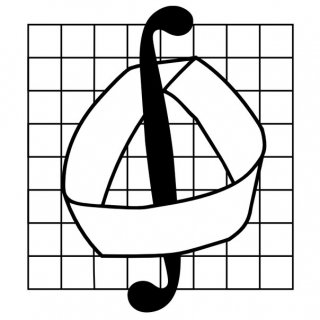
\includegraphics[scale=1]{mm_logo} \\[0.6cm]

{\bf \normalsize Численное моделирование нестационарного течения газа с использованием неявной разностной схемы А.Г.Соколова СКОРОСТЬ-ПЛОТНОСТЬ}\\[0.5cm]

\end{center}

\vspace{1.5cm}
\begin{flushright}
{\bfРаботу выполнил:}\\
студент 410 группы Ясинский Н. Д.\\[0.5cm]
\vspace{1cm}
\end{flushright}

\end{titlepage}

\tableofcontents

\section {Постановка задачи}
Рассмотрим систему уравнений, описывающую нестационарное движение баротропного газа в области $\Omega = \Omega_{00} \cup \Omega_{01} \cup \Omega_{02} \cup \Omega_{11} \cup \Omega_{20} \cup \Omega_{21} \cup \Omega_{22}$, где $\Omega_{nm}$ - квадрат $n < x < n + 1$ и $m < y < m + 1$:

\begin{equation}
 \begin{cases}
   \frac{\partial \rho}{\partial t} + div(\rho \boldsymbol{u}) = 0,
   \\
   \rho [\frac{\partial \boldsymbol{u}}{\partial t} + (\boldsymbol{u}, \nabla)\boldsymbol{u}] +\nabla p = L\boldsymbol{u} + \rho \boldsymbol{f},
   \\
   p = p(\rho),
 \end{cases}
\end{equation} 
где $L$ есть линейный симметричный положительно определенный оператор. В нашей задаче берем 

$$ 
L\boldsymbol{u} \equiv div(\mu \nabla \boldsymbol{u}) + \frac{1}{3} \nabla(\mu div\boldsymbol{u})
$$

Как и в одномерном случае, через $\mu$ обозначаем известную константу (0.1, 0.01 или 0.001), давление газа полагаем равным $p = C\rho$, где C = 1, 100, 1000. Вектор внешних сил $\boldsymbol{f} = \boldsymbol{f} (\boldsymbol{x})$ считаем заданным.

Поскольку мы рассматриваем двумерную по пространству задачу, то напишем уравнения системы в этом случае:
\begin{equation}
 \begin{cases}
   \frac{\partial \rho}{\partial t} + \frac{\partial \rho u_1}{\partial x_1} + \frac{\partial \rho u_2}{\partial x_2} = f_0,
   \\
   \frac{\partial \rho u_1}{\partial t} + \frac{\partial \rho u_1^2}{\partial x_1} + \frac{\partial \rho u_2 u_1}{\partial x_2} + \frac{\partial p}{\partial x_1} = \mu (\frac{4}{3}\frac{\partial^2 u_1}{\partial x_1^2} + \frac{\partial^2 u_1}{\partial x_2^2} + \frac{1}{3}\frac{\partial^2 u_2}{\partial x_1 \partial x_2}) + \rho f_1
   \\
   \frac{\partial \rho u_2}{\partial t} + \frac{\partial \rho u_2^2}{\partial x_2} + \frac{\partial \rho u_1 u_2}{\partial x_1} + \frac{\partial p}{\partial x_2} = \mu (\frac{4}{3}\frac{\partial^2 u_2}{\partial x_2^2} + \frac{\partial^2 u_2}{\partial x_1^2} + \frac{1}{3}\frac{\partial^2 u_1}{\partial x_1 \partial x_2}) + \rho f_2
 \end{cases}
\end{equation} 

Неизвестные функции: плотность $\rho$ и вектор скорости $\boldsymbol{u}$ являются функциями переменных Эйлера $(t, \boldsymbol{x}) \in Q = [0, T] \times \Omega $

В начальный момент времени задаются функции, значения которых определяют плотность и скорость газа в каждой точке $\Omega$:
$$
(\rho, \boldsymbol{u})|_{t=0} = (\rho_0, \boldsymbol{u_0}),\ x \in \Omega. \\
$$

Наконец, установим граничные условия прилипания газа: ${u_1}|_{\partial \Omega} = {u_2}|_{\partial \Omega} = 0$

\section {Разностная схема}

Для поиска численного решения задачи можно использовать схему А.Г.Соколова СКОРОСТЬ-ПЛОТНОСТЬ.

\begin{equation}
\begin{cases}
H_{\bar{s_1} \bar{s_2}}V_{1_t} + H_{\bar{s_1} \bar{s_2}}\delta_1\{\hat{V_1}, V_1\} + H_{\bar{s_1} \bar{s_2}}\delta_2\{\hat{V_1}, V_2\} + p(H_{\bar{s_2}})\bar{x_1} = \\
 = \mu(\frac{4}{3}(\hat{V_1})_{x_1\bar{x_1}} + (\hat{V_1})_{x_2\bar{x_2}}) + \frac{\mu}{3}(V_2)_{\stackrel{o}{x_1} \stackrel{o}{x_2}} + f_1H_{\bar{s_1} \bar{s_2}},\; \text{при}\; H_{\bar{s_1} \bar{s_2}} \ne 0,  \\ 
 \hat{V_1} = 0,\; \text{при}\; H_{\bar{s_1} \bar{s_2}} = 0,\ \boldsymbol{x} \in \Omega_{\bar{h}}; \\
 
 H_{\bar{s_1} \bar{s_2}}V_{2_t} + H_{\bar{s_1} \bar{s_2}}\delta_1\{\hat{V_2}, V_1\} + H_{\bar{s_1} \bar{s_2}}\delta_2\{\hat{V_2}, V_2\} + p(H_{\bar{s_1}})\bar{x_2} = \\
 = \mu(\frac{4}{3}(\hat{V_2})_{x_2\bar{x_2}} + (\hat{V_2})_{x_1\bar{x_1}}) + \frac{\mu}{3}(V_1)_{\stackrel{o}{x_1} \stackrel{o}{x_2}} + f_2H_{\bar{s_1} \bar{s_2}},\; \text{при}\; H_{\bar{s_1} \bar{s_2}} \ne 0,  \\ 
 \hat{V_2} = 0,\; \text{при}\; H_{\bar{s_1} \bar{s_2}} = 0,\ \boldsymbol{x} \in \Omega_{\bar{h}}; \\
 
 H_t + (\sigma_1\{\hat{H}, \hat{V}_{1_{s_2}}\}\hat{V}_{1_{s_2}})_{x_1} + (\sigma_2\{\hat{H}, \hat{V}_{2_{s_1}}\}\hat{V}_{2_{s_1}})_{x_2} = 0,\ \boldsymbol{x} \in \Omega_{\bar{h}}^\frac{1}{2}
 \end{cases}
\end{equation} 

\section {Запись уравнений разностной схемы в координатах}

\noindent Используем следующие обозначения: 

$\tilde{H}_{m_1, m_2}^{n} = \frac{H_{m_1, m_2}^{n}+H_{m_1-1, m_2}^{n}+H_{m_1, m_2-1}^{n}+H_{m_1-1, m_2-1}^{n}}{4}$,
 
$\ \tilde{V}_{1_{m_1, m_2}}^{n} = \frac{V_{1_{m_1, m_2}}^{n} + V_{1_{m_1, m_2+1}}^{n}}{2}$,
$\ \tilde{V}_{2_{m_1, m_2}}^{n} = \frac{V_{2_{m_1, m_2}}^{n} + V_{2_{m_1+1, m_2}}^{n}}{2}$, 

$\ H_{1_{m_1, m_2}}^{n} = \frac{H_{m_1, m_2}^{n} + H_{m_1, m_2-1}^{n}}{2}$, 
$\ H_{2_{m_1, m_2}}^{n} = \frac{H_{m_1, m_2}^{n} + H_{m_1-1, m_2}^{n}}{2}$.

\noindent Тогда первое уравнение разностной схемы в координатах выглядит так:
\begin{equation}
\begin{cases}
V_{1_{m_1, m_2}}^{n+1} (\tilde{H}_{m_1, m_2}^{n} (\frac{1}{\tau} + \frac{|V_{1_{m_1, m_2}}^{n}|}{\h_1} + \frac{|V_{2_{m_1, m_2}}^{n}|}{\h_2}) + \frac{8\mu}{3h_1^2} + \frac{2\mu}{h_2^2})\ + \\
+\ V_{1_{m_1 - 1, m_2}}^{n+1} (-\frac{\tilde{H}_{m_1, m_2}^{n}}{2h_1} (|V_{1_{m_1, m_2}}^{n}| + V_{1_{m_1, m_2}}^{n}) - \frac{4\mu}{3h_1^2}) + V_{1_{m_1, m_2 - 1}}^{n+1} (-\frac{\tilde{H}_{m_1, m_2}^{n}}{2h_2} (|V_{2_{m_1, m_2}}^{n}| + V_{2_{m_1, m_2}}^{n}) - \frac{\mu}{h_2^2})\ + \\
+\ V_{1_{m_1 + 1, m_2}}^{n+1} (-\frac{\tilde{H}_{m_1, m_2}^{n}}{2h_1} (|V_{1_{m_1, m_2}}^{n}| - V_{1_{m_1, m_2}}^{n}) - \frac{4\mu}{3h_1^2}) + V_{1_{m_1, m_2 + 1}}^{n+1} (-\frac{\tilde{H}_{m_1, m_2}^{n}}{2h_2} (|V_{2_{m_1, m_2}}^{n}| - V_{2_{m_1, m_2}}^{n}) - \frac{\mu}{h_2^2}) = \\
=\ \frac{\tilde{H}_{m_1, m_2}^{n} V_{1_{m_1, m_2}}^{n}}{\tau} - \frac{p(H_{1_{m_1, m_2}}^{n})-p(H_{1_{m_1-1, m_2}}^{n})}{h_1} + \frac{\mu}{3} \frac{V_{2_{m_1-1, m_2-1}}^{n} - V_{2_{m_1-1, m_2+1}}^{n} - V_{2_{m_1+1, m_2-1}}^{n} + V_{2_{m_1+1, m_2+1}}^{n}}{4h_1 h_2}\ + \\
+\ f_{1_{m_1, m_2}}^{n+1} \tilde{H}_{m_1, m_2}^{n}\; \text{при}\; \tilde{H}_{m_1, m_2}^{n} \ne 0,\; \text{иначе}\; V_{1_{m_1, m_2}}^{n+1} = 0,\ \boldsymbol{x} \in \Omega_{\bar{h}}.
\end{cases}
\end{equation} 

\noindent Второе уравнение:
\begin{equation}
\begin{cases}
V_{2_{m_1, m_2}}^{n+1} (\tilde{H}_{m_1, m_2}^{n} (\frac{1}{\tau} + \frac{|V_{1_{m_1, m_2}}^{n}|}{\h_1} + \frac{|V_{2_{m_1, m_2}}^{n}|}{\h_2}) + \frac{8\mu}{3h_2^2} + \frac{2\mu}{h_1^2})\ + \\
+\ V_{2_{m_1 - 1, m_2}}^{n+1} (-\frac{\tilde{H}_{m_1, m_2}^{n}}{2h_1} (|V_{1_{m_1, m_2}}^{n}| + V_{1_{m_1, m_2}}^{n}) - \frac{\mu}{h_1^2}) + V_{2_{m_1, m_2 - 1}}^{n+1} (-\frac{\tilde{H}_{m_1, m_2}^{n}}{2h_2} (|V_{2_{m_1, m_2}}^{n}| + V_{2_{m_1, m_2}}^{n}) - \frac{4\mu}{3h_2^2})\ + \\
+\ V_{2_{m_1 + 1, m_2}}^{n+1} (-\frac{\tilde{H}_{m_1, m_2}^{n}}{2h_1} (|V_{1_{m_1, m_2}}^{n}| - V_{1_{m_1, m_2}}^{n}) - \frac{\mu}{h_1^2}) + V_{2_{m_1, m_2 + 1}}^{n+1} (-\frac{\tilde{H}_{m_1, m_2}^{n}}{2h_2} (|V_{2_{m_1, m_2}}^{n}| - V_{2_{m_1, m_2}}^{n}) - \frac{4\mu}{3h_2^2}) = \\
=\ \frac{\tilde{H}_{m_1, m_2}^{n} V_{2_{m_1, m_2}}^{n}}{\tau} - \frac{p(H_{2_{m_1, m_2}}^{n})-p(H_{2_{m_1, m_2-1}}^{n})}{h_2} + \frac{\mu}{3} \frac{V_{1_{m_1-1, m_2-1}}^{n} - V_{1_{m_1-1, m_2+1}}^{n} - V_{1_{m_1+1, m_2-1}}^{n} + V_{1_{m_1+1, m_2+1}}^{n}}{4h_1 h_2}\ + \\
+\ f_{2_{m_1, m_2}}^{n+1} \tilde{H}_{m_1, m_2}^{n}\; \text{при}\; \tilde{H}_{m_1, m_2}^{n} \ne 0,\; \text{иначе}\; V_{2_{m_1, m_2}}^{n+1} = 0,\ \boldsymbol{x} \in \Omega_{\bar{h}}.
\end{cases}
\end{equation} 

\noindent Третье уравнение:
\begin{equation}
\begin{cases}
H_{m_1, m_2}^{n+1} (\frac{1}{\tau} + \frac{1}{2h_1} (\tilde{V}_{1_{m_1+1, m_2}}^{n+1} + |\tilde{V}_{1_{m_1+1, m_2}}^{n+1}| - \tilde{V}_{1_{m_1, m_2}}^{n+1} + |\tilde{V}_{1_{m_1, m_2}}^{n+1}|)\ + \\
+\ \frac{1}{2h_2} (\tilde{V}_{2_{m_1, m_2+1}}^{n+1} + |\tilde{V}_{2_{m_1, m_2+1}}^{n+1}| - \tilde{V}_{2_{m_1, m_2}}^{n+1} + |\tilde{V}_{2_{m_1, m_2}}^{n+1}|))\ + \\
+\ H_{m_1 - 1, m_2}^{n+1} (-\frac{\tilde{V}_{1_{m_1, m_2}}^{n+1} + |\tilde{V}_{1_{m_1, m_2}}^{n+1}|}{2h_1}) + H_{m_1, m_2 - 1}^{n+1} (-\frac{\tilde{V}_{2_{m_1, m_2}}^{n+1} + |\tilde{V}_{2_{m_1, m_2}}^{n+1}|}{2h_2})\ + \\
+\ H_{m_1 + 1, m_2}^{n+1} (\frac{\tilde{V}_{1_{m_1+1, m_2}}^{n+1} - |\tilde{V}_{1_{m_1+1, m_2}}^{n+1}|}{2h_1}) + H_{m_1, m_2 + 1}^{n+1} (\frac{\tilde{V}_{2_{m_1, m_2+1}}^{n+1} - |\tilde{V}_{2_{m_1, m_2+1}}^{n+1}|}{2h_2})\ = \frac{H_{m_1, m_2}^{n}}{\tau} + f_0,\ \boldsymbol{x} \in \Omega_{\bar{h}}^\frac{1}{2}.
\end{cases}
\end{equation} 

На каждом временном слое будем сначала из первых двух уравнений находить $V_{1_{i,j}}$ и $V_{2_{i,j}}$ и далее использовать найденные значения скоростей для нахождения плотности $H_{i,j}$.

\section {Отладка на гладком решении}

Зададим функции:
\begin{gather*}
u_1 = sin(2\pi x_1)sin(2\pi x_2)e^t \\
u_2 = sin(2\pi x_1)sin(2\pi x_2)e^{-t} \\
\rho(t, x_1, x_2) = (cos(2\pi x_1) + \frac{3}{2})(sin(2\pi x_2) + \frac{3}{2})e^t
\end{gather*}

Определим $f_0, f_1, f_2$ так, чтобы они удовлетворяли системе (2) и найдем их непосредственной подстановкой:

\begin{equation}
 \begin{cases}
   u_{1_t} = u_1 \\
   u_{1_{x_1}} = 2\pi cos(2\pi x_1) sin(2\pi x_2)e^t \\
   u_{1_{x_2}} = 2\pi sin(2\pi x_1) cos(2\pi x_2)e^t \\
   u_{1_{x_1, x_1}} = u_{1_{x_2, x_2}} = -4\pi^2 u_1 \\
   u_{1_{x_1, x_2}} = 4\pi^2 cos(2\pi x_1) cos(2\pi x_2)e^t \\
   u_{2_t} = -u_2 \\
   u_{2_{x_1}} = 2\pi cos(2\pi x_1) sin(2\pi x_2)e^{-t} \\
   u_{2_{x_2}} = 2\pi sin(2\pi x_1) cos(2\pi x_2)e^{-t} \\
   u_{2_{x_1, x_1}} = u_{2_{x_2, x_2}} = -4\pi^2 u_2 \\
   u_{2_{x_1, x_2}} = 4\pi^2 cos(2\pi x_1) cos(2\pi x_2)e^{-t} \\
   \rho_t = \rho \\
   \rho_{x_1} = -2\pi sin(2\pi x_1)(sin(2\pi x_2) + \frac{3}{2})e^t \\
   \rho_{x_2} = 2\pi (cos(2\pi x_1) + \frac{3}{2})cos(2\pi x_2)e^t \\
   f_0 = \rho_t + u_1 \rho_{x_1} + \rho u_{1_{x_1}} + u_2 \rho_{x_2} + \rho u_{2_{x_2}} \\
   f_1 = \frac{u_1 \rho_t + \rho u_{1_t} + u_1^2 \rho_{x_1} + 2\rho u_1 u_{1_{x_1}} + u_1 u_2 \rho_{x_2} + u_1 \rho u_{2_{x_2}} + u_2 \rho u_{1_{x_2}} + p_{x_1} - \frac{4}{3}\mu u_{1_{x_1, x_1}} - \mu u_{1_{x_2, x_2}} - \frac{1}{3} \mu u_{2_{x_1, x_2}}}{\rho} \\
   f_2 = \frac{u_2 \rho_t + \rho u_{2_t} + u_2^2 \rho_{x_2} + 2\rho u_2 u_{2_{x_2}} + u_1 u_2 \rho_{x_1} + u_1 \rho u_{2_{x_1}} + u_2 \rho u_{1_{x_1}} + p_{x_2} - \frac{4}{3}\mu u_{2_{x_2, x_2}} - \mu u_{2_{x_1, x_1}} - \frac{1}{3} \mu u_{1_{x_1, x_2}}}{\rho}
 \end{cases}
\end{equation} 

Запустим программу и составим таблицы ошибок численного решения для плотности и скорости в нормах $\|\cdot \|_{C_h},\ \| \cdot \|_{L2},\ \| \cdot \|_W$ при различных значениях $C = 1,\ 10$ и $\mu = 0.1,\ 0.01,\ 0.001.$

\begin{table}[H]
\small
\caption{Ошибка для $H$ при $\mu=0.1$ и $C = 1$}
\begin{center}
\begin{tabular}{|c|c|c|c|c|}
\hline
$\tau$ / h & 0.05 & 0.025 & 0.0125 & 0.00625 \\
\hline
0.050000 & 3.382585e-01  & 2.922250e-01  & 2.847450e-01  & 2.840030e-01 \\
 & 3.058462e-01  & 2.992953e-01  & 3.053588e-01  & 3.108551e-01 \\
 & 2.590994e+01  & 3.230783e+01  & 4.380752e+01  & 6.099383e+01 \\
\hline
0.025000 & 1.951517e-01  & 1.481547e-01  & 1.373600e-01  & 1.358182e-01 \\
 & 1.661374e-01  & 1.476231e-01  & 1.483555e-01  & 1.517066e-01 \\
 & 2.157172e+01  & 2.397083e+01  & 3.082853e+01  & 4.254339e+01 \\
\hline
0.012500 & 1.264181e-01  & 7.670930e-02  & 6.546455e-02  & 6.307194e-02 \\
 & 1.097124e-01  & 7.928331e-02  & 7.285834e-02  & 7.346984e-02 \\
 & 1.993576e+01  & 1.986318e+01  & 2.241246e+01  & 2.957164e+01 \\
\hline
0.006250 & 9.369401e-02  & 6.442703e-02  & 4.256141e-02  & 2.833280e-02 \\
 & 9.241624e-02  & 5.531793e-02  & 4.019941e-02  & 3.625986e-02 \\
 & 1.944743e+01  & 1.856775e+01  & 1.815391e+01  & 2.088751e+01 \\
\hline
\end{tabular}
\end{center}
\end{table}

\begin{table}[H]
\small
\caption{Ошибка для $V_1$ при $\mu=0.1$ и $C = 1$}
\begin{center}
\begin{tabular}{|c|c|c|c|c|}
\hline
$\tau$ / h & 0.05 & 0.025 & 0.0125 & 0.00625 \\
\hline
0.050000 & 3.601637e-01  & 1.314280e-01  & 9.133186e-02  & 7.452318e-02 \\
 & 4.246110e-01  & 1.295482e-01  & 9.116871e-02  & 9.289078e-02 \\
 & 3.037685e+01  & 2.077480e+01  & 2.243616e+01  & 2.717535e+01 \\
\hline
0.025000 & 4.101887e-01  & 9.500941e-02  & 5.117395e-02  & 3.361618e-02 \\
 & 4.515754e-01  & 1.241552e-01  & 4.540428e-02  & 3.658604e-02 \\
 & 3.161865e+01  & 1.995805e+01  & 1.545543e+01  & 1.724373e+01 \\
\hline
0.012500 & 4.352984e-01  & 1.183641e-01  & 3.152034e-02  & 1.379714e-02 \\
 & 4.675480e-01  & 1.313621e-01  & 3.723685e-02  & 1.123091e-02 \\
 & 3.233428e+01  & 2.066203e+01  & 1.358249e+01  & 1.034845e+01 \\
\hline
0.006250 & 4.478783e-01  & 1.300659e-01  & 3.870640e-02  & 1.065004e-02 \\
 & 4.760910e-01  & 1.371567e-01  & 4.080806e-02  & 1.147848e-02 \\
 & 3.271024e+01  & 2.123852e+01  & 1.426613e+01  & 1.026613e+01 \\
\hline
\end{tabular}
\end{center}
\end{table}

\begin{table}[H]
\small
\caption{Ошибка для $V_2$ при $\mu=0.1$ и $C = 1$}
\begin{center}
\begin{tabular}{|c|c|c|c|c|}
\hline
$\tau$ / h & 0.05 & 0.025 & 0.0125 & 0.00625 \\
\hline
0.050000 & 2.460131e-01  & 7.277457e-02  & 3.460319e-02  & 2.562245e-02 \\
 & 2.339442e-01  & 6.682971e-02  & 3.103373e-02  & 2.523181e-02 \\
 & 2.163462e+01  & 1.431885e+01  & 1.228577e+01  & 1.362920e+01 \\
\hline
0.025000 & 2.477339e-01  & 6.508771e-02  & 2.254865e-02  & 1.333730e-02 \\
 & 2.324035e-01  & 6.081065e-02  & 2.032757e-02  & 1.193801e-02 \\
 & 2.160151e+01  & 1.371151e+01  & 9.964773e+00  & 9.384880e+00 \\
\hline
0.012500 & 2.491775e-01  & 6.338530e-02  & 1.808867e-02  & 7.304048e-03 \\
 & 2.318302e-01  & 5.873068e-02  & 1.685523e-02  & 6.593511e-03 \\
 & 2.160445e+01  & 1.357887e+01  & 9.347249e+00  & 7.424938e+00 \\
\hline
0.006250 & 2.498810e-01  & 6.330425e-02  & 1.733863e-02  & 7.571211e-03 \\
 & 2.315967e-01  & 5.797251e-02  & 1.606412e-02  & 5.747964e-03 \\
 & 2.161109e+01  & 1.356425e+01  & 9.349207e+00  & 7.379013e+00 \\
\hline
\end{tabular}
\end{center}
\end{table}

\begin{table}[H]
\small
\caption{Ошибка для $H$ при $\mu=0.01$ и $C = 1$}
\begin{center}
\begin{tabular}{|c|c|c|c|c|}
\hline
$\tau$ / h & 0.05 & 0.025 & 0.0125 & 0.00625 \\
\hline
0.050000 & 4.122917e-01  & 2.812023e-01  & 2.514614e-01  & 2.448973e-01 \\
 & 3.994312e-01  & 3.190713e-01  & 3.074923e-01  & 3.069445e-01 \\
 & 2.995057e+01  & 3.260100e+01  & 4.258987e+01  & 5.874851e+01 \\
\hline
0.025000 & 2.769793e-01  & 1.460063e-01  & 1.155383e-01  & nan \\
 & 2.615796e-01  & 1.656424e-01  & 1.517471e-01  & nan \\
 & 2.544780e+01  & 2.393560e+01  & 2.954906e+01  & nan \\
\hline
0.012500 & 2.096799e-01  & 7.886364e-02  & 5.391509e-02  & 5.298915e-02 \\
 & 2.004414e-01  & 9.098553e-02  & 7.558236e-02  & 7.371939e-02 \\
 & 2.305103e+01  & 1.849456e+01  & 2.056341e+01  & 2.713830e+01 \\
\hline
0.006250 & 1.761250e-01  & 4.783208e-02  & 3.556534e-02  & 3.373939e-02 \\
 & 1.741278e-01  & 5.604922e-02  & 4.002608e-02  & 3.829052e-02 \\
 & 2.184015e+01  & 1.552498e+01  & 1.529783e+01  & 1.893338e+01 \\
\hline
\end{tabular}
\end{center}
\end{table}

\begin{table}[H]
\small
\caption{Ошибка для $V_1$ при $\mu=0.01$ и $C = 1$}
\begin{center}
\begin{tabular}{|c|c|c|c|c|}
\hline
$\tau$ / h & 0.05 & 0.025 & 0.0125 & 0.00625 \\
\hline
0.050000 & 7.726822e-01  & 2.455662e-01  & 9.056710e-02  & 3.982691e-02 \\
 & 9.653279e-01  & 3.293501e-01  & 1.196739e-01  & 4.377673e-02 \\
 & 4.832513e+01  & 3.384282e+01  & 2.481890e+01  & 1.968564e+01 \\
\hline
0.025000 & 8.214596e-01  & 2.895325e-01  & 1.282552e-01  & nan \\
 & 9.927509e-01  & 3.476983e-01  & 1.392235e-01  & nan \\
 & 4.901033e+01  & 3.475919e+01  & 2.667454e+01  & nan \\
\hline
0.012500 & 8.458603e-01  & 3.115743e-01  & 1.494754e-01  & 9.305098e-02 \\
 & 1.007031e+00  & 3.586793e-01  & 1.529832e-01  & 9.297785e-02 \\
 & 4.936799e+01  & 3.532249e+01  & 2.800631e+01  & 2.705763e+01 \\
\hline
0.006250 & 8.580598e-01  & 3.226104e-01  & 1.601039e-01  & 1.034728e-01 \\
 & 1.014309e+00  & 3.645818e-01  & 1.605974e-01  & 1.030919e-01 \\
 & 4.955037e+01  & 3.562650e+01  & 2.872893e+01  & 2.843333e+01 \\
\hline
\end{tabular}
\end{center}
\end{table}

\begin{table}[H]
\small
\caption{Ошибка для $V_2$ при $\mu=0.01$ и $C = 1$}
\begin{center}
\begin{tabular}{|c|c|c|c|c|}
\hline
$\tau$ / h & 0.05 & 0.025 & 0.0125 & 0.00625 \\
\hline
0.050000 & 8.504541e-01  & 2.015802e-01  & 5.956985e-02  & 4.510771e-02 \\
 & 8.462032e-01  & 1.921688e-01  & 5.663115e-02  & 3.325543e-02 \\
 & 4.514841e+01  & 2.813022e+01  & 2.061922e+01  & 1.908164e+01 \\
\hline
0.025000 & 8.484116e-01  & 2.002554e-01  & 7.049868e-02  & nan \\
 & 8.440840e-01  & 1.882500e-01  & 5.917255e-02  & nan \\
 & 4.520644e+01  & 2.820189e+01  & 2.128681e+01  & nan \\
\hline
0.012500 & 8.472332e-01  & 2.012441e-01  & 7.620237e-02  & 6.092131e-02 \\
 & 8.431215e-01  & 1.868970e-01  & 6.247501e-02  & 5.066535e-02 \\
 & 4.524011e+01  & 2.827720e+01  & 2.178233e+01  & 2.203129e+01 \\
\hline
0.006250 & 8.466064e-01  & 2.028664e-01  & 7.905384e-02  & 6.371225e-02 \\
 & 8.426641e-01  & 1.863782e-01  & 6.456430e-02  & 5.444196e-02 \\
 & 4.525801e+01  & 2.832466e+01  & 2.206253e+01  & 2.262367e+01 \\
\hline
\end{tabular}
\end{center}
\end{table}

\begin{table}[H]
\small
\caption{Ошибка для $H$ при $\mu=0.001$ и $C = 1$}
\begin{center}
\begin{tabular}{|c|c|c|c|c|}
\hline
$\tau$ / h & 0.05 & 0.025 & 0.0125 & 0.00625 \\
\hline
0.050000 & 4.359734e-01  & 2.836349e-01  & 3.660001e-01  & 2.462570e+01 \\
 & 4.673008e-01  & 3.338357e-01  & 3.116752e-01  & 3.742721e+00 \\
 & 3.260859e+01  & 3.332512e+01  & 4.476679e+01  & 6.401519e+02 \\
\hline
0.025000 & 3.018430e-01  & 1.508509e-01  & 1.156831e-01  & 1.080348e-01 \\
 & 3.380116e-01  & 1.824690e-01  & 1.558249e-01  & 1.511675e-01 \\
 & 2.883934e+01  & 2.509370e+01  & 2.987060e+01  & 4.038614e+01 \\
\hline
0.012500 & 2.353122e-01  & 9.355749e-02  & 6.327856e-02  & nan \\
 & 2.820088e-01  & 1.101973e-01  & 7.990994e-02  & nan \\
 & 2.695844e+01  & 2.014641e+01  & 2.119039e+01  & nan \\
\hline
0.006250 & 2.047358e-01  & 6.734325e-02  & nan  & nan \\
 & 2.577537e-01  & 7.735284e-02  & nan  & nan \\
 & 2.604453e+01  & 1.754713e+01  & nan  & nan \\
\hline
\end{tabular}
\end{center}
\end{table}

\begin{table}[H]
\small
\caption{Ошибка для $V_1$ при $\mu=0.001$ и $C = 1$}
\begin{center}
\begin{tabular}{|c|c|c|c|c|}
\hline
$\tau$ / h & 0.05 & 0.025 & 0.0125 & 0.00625 \\
\hline
0.050000 & 1.666174e+00  & 7.043645e-01  & 4.684878e-01  & 3.144968e+01 \\
 & 1.503148e+00  & 7.304118e-01  & 4.844502e-01  & 8.323016e+00 \\
 & 6.004914e+01  & 5.052014e+01  & 5.576455e+01  & 9.575495e+02 \\
\hline
0.025000 & 1.699403e+00  & 7.429665e-01  & 5.019025e-01  & 4.176943e-01 \\
 & 1.538692e+00  & 7.575845e-01  & 5.118000e-01  & 4.499569e-01 \\
 & 6.080118e+01  & 5.158499e+01  & 5.248194e+01  & 5.999946e+01 \\
\hline
0.012500 & 1.717114e+00  & 7.630549e-01  & 5.186224e-01  & nan \\
 & 1.561353e+00  & 7.726113e-01  & 5.264785e-01  & nan \\
 & 6.125439e+01  & 5.215625e+01  & 5.325308e+01  & nan \\
\hline
0.006250 & 1.726253e+00  & 7.733053e-01  & nan  & nan \\
 & 1.573984e+00  & 7.804740e-01  & nan  & nan \\
 & 6.150236e+01  & 5.245080e+01  & nan  & nan \\
\hline
\end{tabular}
\end{center}
\end{table}

\begin{table}[H]
\small
\caption{Ошибка для $V_2$ при $\mu=0.001$ и $C = 1$}
\begin{center}
\begin{tabular}{|c|c|c|c|c|}
\hline
$\tau$ / h & 0.05 & 0.025 & 0.0125 & 0.00625 \\
\hline
0.050000 & 1.453296e+00  & 4.643355e-01  & 3.772796e-01  & 8.176351e+00 \\
 & 1.147613e+00  & 3.835316e-01  & 3.739666e-01  & 9.858405e-01 \\
 & 5.303547e+01  & 4.193850e+01  & 5.111102e+01  & 3.112038e+02 \\
\hline
0.025000 & 1.445692e+00  & 4.728937e-01  & 3.866631e-01  & 3.898031e-01 \\
 & 1.153702e+00  & 3.912218e-01  & 3.819731e-01  & 4.000425e-01 \\
 & 5.317349e+01  & 4.232242e+01  & 4.904422e+01  & 5.914669e+01 \\
\hline
0.012500 & 1.440002e+00  & 4.772398e-01  & 3.913910e-01  & nan \\
 & 1.156502e+00  & 3.951769e-01  & 3.864010e-01  & nan \\
 & 5.324462e+01  & 4.251953e+01  & 4.927759e+01  & nan \\
\hline
0.006250 & 1.436669e+00  & 4.794547e-01  & nan  & nan \\
 & 1.157906e+00  & 3.971910e-01  & nan  & nan \\
 & 5.328328e+01  & 4.262017e+01  & nan  & nan \\
\hline
\end{tabular}
\end{center}
\end{table}

\begin{table}[H]
\small
\caption{Ошибка для $H$ при $\mu=0.1$ и $C = 10$}
\begin{center}
\begin{tabular}{|c|c|c|c|c|}
\hline
$\tau$ / h & 0.05 & 0.025 & 0.0125 & 0.00625 \\
\hline
0.050000 & 4.379158e-01  & 3.088312e-01  & 2.795949e-01  & 2.737192e-01 \\
 & 4.095019e-01  & 3.260409e-01  & 3.136366e-01  & 3.129914e-01 \\
 & 3.060367e+01  & 3.364110e+01  & 4.399431e+01  & 6.064656e+01 \\
\hline
0.025000 & 3.010068e-01  & 1.719869e-01  & 1.420741e-01  & nan \\
 & 2.724374e-01  & 1.723619e-01  & 1.568701e-01  & nan \\
 & 2.614531e+01  & 2.518130e+01  & 3.130805e+01  & nan \\
\hline
0.012500 & 2.329619e-01  & 1.040855e-01  & 7.373151e-02  & nan \\
 & 2.118628e-01  & 9.759850e-02  & 7.917247e-02  & nan \\
 & 2.376315e+01  & 1.985254e+01  & 2.256677e+01  & nan \\
\hline
0.006250 & 1.990453e-01  & 7.024033e-02  & nan  & 3.271347e-02 \\
 & 1.857565e-01  & 6.243194e-02  & nan  & 3.789985e-02 \\
 & 2.255067e+01  & 1.678784e+01  & nan  & 2.115671e+01 \\
\hline
\end{tabular}
\end{center}
\end{table}

\begin{table}[H]
\small
\caption{Ошибка для $V_1$ при $\mu=0.1$ и $C = 10$}
\begin{center}
\begin{tabular}{|c|c|c|c|c|}
\hline
$\tau$ / h & 0.05 & 0.025 & 0.0125 & 0.00625 \\
\hline
0.050000 & 7.204431e-01  & 3.116563e-01  & 1.685392e-01  & 1.061471e-01 \\
 & 9.770114e-01  & 3.509234e-01  & 1.582984e-01  & 9.953150e-02 \\
 & 4.842439e+01  & 3.491748e+01  & 2.869366e+01  & 2.795485e+01 \\
\hline
0.025000 & 7.690490e-01  & 2.912625e-01  & 1.426778e-01  & nan \\
 & 9.987966e-01  & 3.560184e-01  & 1.471959e-01  & nan \\
 & 4.897149e+01  & 3.502905e+01  & 2.716655e+01  & nan \\
\hline
0.012500 & 7.934429e-01  & 2.814438e-01  & 1.304680e-01  & nan \\
 & 1.010494e+00  & 3.608143e-01  & 1.467062e-01  & nan \\
 & 4.926667e+01  & 3.522359e+01  & 2.692458e+01  & nan \\
\hline
0.006250 & 8.056646e-01  & 2.765132e-01  & nan  & 5.766870e-02 \\
 & 1.016536e+00  & 3.637599e-01  & nan  & 6.457842e-02 \\
 & 4.941936e+01  & 3.535443e+01  & nan  & 2.137451e+01 \\
\hline
\end{tabular}
\end{center}
\end{table}

\begin{table}[H]
\small
\caption{Ошибка для $V_2$ при $\mu=0.1$ и $C = 10$}
\begin{center}
\begin{tabular}{|c|c|c|c|c|}
\hline
$\tau$ / h & 0.05 & 0.025 & 0.0125 & 0.00625 \\
\hline
0.050000 & 8.779638e-01  & 2.341308e-01  & 8.521627e-02  & 4.990941e-02 \\
 & 8.755831e-01  & 2.176451e-01  & 7.441395e-02  & 4.091681e-02 \\
 & 4.550631e+01  & 2.860092e+01  & 2.065922e+01  & 1.823011e+01 \\
\hline
0.025000 & 8.774487e-01  & 2.257516e-01  & 7.314089e-02  & nan \\
 & 8.733826e-01  & 2.100133e-01  & 6.354602e-02  & nan \\
 & 4.554308e+01  & 2.839343e+01  & 1.978960e+01  & nan \\
\hline
0.012500 & 8.771238e-01  & 2.216494e-01  & 6.828953e-02  & nan \\
 & 8.723749e-01  & 2.066381e-01  & 5.945652e-02  & nan \\
 & 4.556552e+01  & 2.832600e+01  & 1.955954e+01  & nan \\
\hline
0.006250 & 8.769438e-01  & 2.195770e-01  & nan  & 2.201314e-02 \\
 & 8.718950e-01  & 2.050710e-01  & nan  & 1.969993e-02 \\
 & 4.557777e+01  & 2.830187e+01  & nan  & 1.480412e+01 \\
\hline
\end{tabular}
\end{center}
\end{table}

\begin{table}[H]
\small
\caption{Ошибка для $H$ при $\mu=0.01$ и $C = 10$}
\begin{center}
\begin{tabular}{|c|c|c|c|c|}
\hline
$\tau$ / h & 0.05 & 0.025 & 0.0125 & 0.00625 \\
\hline
0.050000 & 5.022297e-01  & 2.318006e+01  & 8.002827e+01  & 4.569114e+02 \\
 & 4.983093e-01  & 4.033700e+00  & 1.255065e+01  & 2.718427e+01 \\
 & 3.425143e+01  & 2.526827e+02  & 6.479960e+02  & 1.625057e+03 \\
\hline
0.025000 & 3.667539e-01  & 1.889509e-01  & 1.448961e-01  & 1.346814e-01 \\
 & 3.709241e-01  & 1.962107e-01  & 1.633320e-01  & 1.571070e-01 \\
 & 3.052235e+01  & 2.698553e+01  & 3.190348e+01  & 4.284493e+01 \\
\hline
0.012500 & 2.993979e-01  & 1.217692e-01  & 7.748501e-02  & 6.719677e-02 \\
 & 3.155665e-01  & 1.246295e-01  & 8.610734e-02  & 7.898373e-02 \\
 & 2.860323e+01  & 2.219031e+01  & 2.341771e+01  & 3.035203e+01 \\
\hline
0.006250 & 2.658226e-01  & 8.828099e-02  & 4.388522e-02  & 3.355768e-02 \\
 & 2.913040e-01  & 9.213179e-02  & 4.816854e-02  & 4.008584e-02 \\
 & 2.764170e+01  & 1.951889e+01  & 1.780842e+01  & 2.159109e+01 \\
\hline
\end{tabular}
\end{center}
\end{table}

\begin{table}[H]
\small
\caption{Ошибка для $V_1$ при $\mu=0.01$ и $C = 10$}
\begin{center}
\begin{tabular}{|c|c|c|c|c|}
\hline
$\tau$ / h & 0.05 & 0.025 & 0.0125 & 0.00625 \\
\hline
0.050000 & 1.359984e+00  & 9.816287e+01  & 3.730740e+02  & 7.263507e+02 \\
 & 1.314541e+00  & 3.006015e+01  & 9.733602e+01  & 1.527184e+02 \\
 & 5.786361e+01  & 6.794086e+02  & 1.636865e+03  & 2.854633e+03 \\
\hline
0.025000 & 1.400920e+00  & 4.422100e-01  & 1.728284e-01  & 8.584164e-02 \\
 & 1.339660e+00  & 4.856445e-01  & 2.112132e-01  & 1.059539e-01 \\
 & 5.843342e+01  & 4.147836e+01  & 3.231285e+01  & 2.716561e+01 \\
\hline
0.012500 & 1.421356e+00  & 4.605578e-01  & 1.900734e-01  & 1.047909e-01 \\
 & 1.352040e+00  & 4.934495e-01  & 2.181868e-01  & 1.144532e-01 \\
 & 5.871929e+01  & 4.181827e+01  & 3.285871e+01  & 2.834385e+01 \\
\hline
0.006250 & 1.431589e+00  & 4.697625e-01  & 1.988547e-01  & 1.144009e-01 \\
 & 1.358144e+00  & 4.976405e-01  & 2.223616e-01  & 1.198970e-01 \\
 & 5.886130e+01  & 4.200244e+01  & 3.319438e+01  & 2.909968e+01 \\
\hline
\end{tabular}
\end{center}
\end{table}

\begin{table}[H]
\small
\caption{Ошибка для $V_2$ при $\mu=0.01$ и $C = 10$}
\begin{center}
\begin{tabular}{|c|c|c|c|c|}
\hline
$\tau$ / h & 0.05 & 0.025 & 0.0125 & 0.00625 \\
\hline
0.050000 & 1.680875e+00  & 6.494087e+01  & 2.248977e+02  & 6.399047e+02 \\
 & 1.419798e+00  & 1.078925e+01  & 6.382032e+01  & 1.363810e+02 \\
 & 5.627146e+01  & 4.154757e+02  & 1.273870e+03  & 2.628431e+03 \\
\hline
0.025000 & 1.679677e+00  & 4.179273e-01  & 1.031969e-01  & 6.266666e-02 \\
 & 1.422674e+00  & 3.110594e-01  & 8.817872e-02  & 5.281883e-02 \\
 & 5.638024e+01  & 3.400912e+01  & 2.485517e+01  & 2.349406e+01 \\
\hline
0.012500 & 1.678966e+00  & 4.131386e-01  & 9.866717e-02  & 7.059630e-02 \\
 & 1.424404e+00  & 3.092335e-01  & 8.951032e-02  & 5.924689e-02 \\
 & 5.644265e+01  & 3.401329e+01  & 2.512959e+01  & 2.442240e+01 \\
\hline
0.006250 & 1.678427e+00  & 4.106807e-01  & 9.638085e-02  & 7.471750e-02 \\
 & 1.425261e+00  & 3.083945e-01  & 9.050876e-02  & 6.272706e-02 \\
 & 5.647419e+01  & 3.402114e+01  & 2.529399e+01  & 2.491654e+01 \\
\hline
\end{tabular}
\end{center}
\end{table}

\begin{table}[H]
\small
\caption{Ошибка для $H$ при $\mu=0.001$ и $C = 10$}
\begin{center}
\begin{tabular}{|c|c|c|c|c|}
\hline
$\tau$ / h & 0.05 & 0.025 & 0.0125 & 0.00625 \\
\hline
0.050000 & 1.619038e+01  & 2.132490e+02  & 1.833493e+03  & nan \\
 & 8.086971e+00  & 2.917370e+01  & 7.611850e+01  & nan \\
 & 2.175257e+02  & 6.256078e+02  & 1.747229e+03  & nan \\
\hline
0.025000 & 4.157885e-01  & 1.294371e+01  & 6.110039e+02  & nan \\
 & 4.089933e-01  & 5.336948e+00  & 3.034687e+01  & nan \\
 & 3.195356e+01  & 2.929706e+02  & 1.064212e+03  & nan \\
\hline
0.012500 & 3.450884e-01  & 1.345620e-01  & 1.446227e+01  & nan \\
 & 3.513142e-01  & 1.351194e-01  & 4.452185e+00  & nan \\
 & 2.999332e+01  & 2.319011e+01  & 4.480412e+02  & nan \\
\hline
0.006250 & 3.099180e-01  & 1.015528e-01  & 4.685647e-02  & nan \\
 & 3.262885e-01  & 1.036259e-01  & 5.069289e-02  & nan \\
 & 2.902492e+01  & 2.067521e+01  & 1.835243e+01  & nan \\
\hline
\end{tabular}
\end{center}
\end{table}

\begin{table}[H]
\small
\caption{Ошибка для $V_1$ при $\mu=0.001$ и $C = 10$}
\begin{center}
\begin{tabular}{|c|c|c|c|c|}
\hline
$\tau$ / h & 0.05 & 0.025 & 0.0125 & 0.00625 \\
\hline
0.050000 & 2.592893e+02  & 9.188390e+02  & 2.046037e+03  & nan \\
 & 2.482567e+02  & 5.788986e+02  & 8.298532e+02  & nan \\
 & 1.142722e+03  & 2.247511e+03  & 3.898030e+03  & nan \\
\hline
0.025000 & 3.261186e+00  & 3.658394e+02  & 8.167039e+02  & nan \\
 & 2.934761e+00  & 2.079971e+02  & 5.741028e+02  & nan \\
 & 8.312269e+01  & 1.476630e+03  & 3.148327e+03  & nan \\
\hline
0.012500 & 3.352350e+00  & 7.989225e-01  & 2.038734e+02  & nan \\
 & 3.041358e+00  & 7.646975e-01  & 1.511962e+02  & nan \\
 & 8.376787e+01  & 5.322959e+01  & 1.871809e+03  & nan \\
\hline
0.006250 & 3.348656e+00  & 8.096317e-01  & 5.078112e-01  & nan \\
 & 3.058518e+00  & 7.769644e-01  & 5.215247e-01  & nan \\
 & 8.384589e+01  & 5.363803e+01  & 5.272447e+01  & nan \\
\hline
\end{tabular}
\end{center}
\end{table}

\begin{table}[H]
\small
\caption{Ошибка для $V_2$ при $\mu=0.001$ и $C = 10$}
\begin{center}
\begin{tabular}{|c|c|c|c|c|}
\hline
$\tau$ / h & 0.05 & 0.025 & 0.0125 & 0.00625 \\
\hline
0.050000 & 3.097526e+02  & 9.105192e+02  & 1.810486e+03  & nan \\
 & 2.465527e+02  & 6.508973e+02  & 9.003029e+02  & nan \\
 & 1.145382e+03  & 2.222291e+03  & 3.831220e+03  & nan \\
\hline
0.025000 & 3.800390e+00  & 3.093700e+02  & 9.076518e+02  & nan \\
 & 2.869558e+00  & 2.030082e+02  & 5.383942e+02  & nan \\
 & 8.138894e+01  & 1.426623e+03  & 3.115168e+03  & nan \\
\hline
0.012500 & 3.762316e+00  & 6.709359e-01  & 2.116510e+02  & nan \\
 & 2.881800e+00  & 5.676468e-01  & 1.526669e+02  & nan \\
 & 8.138077e+01  & 4.663713e+01  & 1.858727e+03  & nan \\
\hline
0.006250 & 3.766894e+00  & 6.714674e-01  & 3.888786e-01  & nan \\
 & 2.880976e+00  & 5.676194e-01  & 4.049462e-01  & nan \\
 & 8.128286e+01  & 4.660626e+01  & 5.027010e+01  & nan \\
\hline
\end{tabular}
\end{center}
\end{table}

\end{document}
